\documentclass{article}
\usepackage[utf8]{inputenc}
\usepackage{graphicx}

\title{Website Storyboard}
\date{September 2020}

% ------------
% DOCUMENT
% ------------
\begin{document}
    \begin{flushright}
        CSE 321 Website Storyboard
    \end{flushright}
    
    \begin{enumerate}
        \item[\textbf{Theme}:]
        Ice Breakr - A dating website that puts the conversation first.\\
    
        \item[\textbf{Group Name}:]
        Dream Machine\\
        Group #9\\
    
        \item[\textbf{Members}:]
        Logan Decker, Pierce Mayadag, Wesley Pick-Roth\\
    
        \item[\textbf{Background}:]
        When comparing the experiences of each members with websites and apps that we felt could use improvements, we determined that many dating sites tend to have similar problems that the conversations don't go anywhere, or that people feel shallow scrolling through and judging others based on their looks. So we decided to dedicate ourselves to creating a dating site that puts meaningful conversation and connection first, and people can gradually unlock additional interests and information as they talk more.\\
    
        \item[\textbf{Relevant Websites}]
            :Most standard dating websites require users to create a profile by filling out personal information which will then be used to match that user with another user that has related interests and characteristics.
            \begin{enumerate}
                \item[Tinder -]
                A quick and easy-to-use dating site with a focus on more immediate relationships and a minimal design.\\
                
                \item[Bumble -]
                A dating site where women make the first move. Focuses on user initiative by letting users choose the exact kind of relationship they want.\\
                
                \item[Hinge -]
                A dating site where the emphasis is on the user profiles. Tries to make long-lasting matches.\\
                
                \item[Plenty of Fish -]
                A typical dating site. Doesn't really try to focus in on anything.\\
                
                \item[OkCupid -]
                A dating site where matching is highly user-driven (users can look for very specific traits in partners).\\
            \end{enumerate}
        
        \item[\textbf{Desired Features}:]
        Users must 'unlock' information about a matching user by doing things like having a conversation in order to see user photos. Users will need to enter their location so as to try and match them with other users that are nearby. Users should be shown other potential matches one-at-a-time to try and avoid overloading the user with information. Users will need to enter the kind of relationship that they're looking for in order to better match them, for example, "looking for a short term relationship" or "looking for a lifelong partner". Users will need to fill out the answers to several questions in order to better match them, such as "What job do you have?" or "What do you like to do in your free time?". Our site will filter potential matches with user-specified age and distance filters, and, on the back end, match users with shared interests and information. Users will need to come up with topics of conversation or conversation starters that they find important so as to promote the initial conversation in a match.\\
    \end{enumerate}
    \hspace{-2cm}\begin{tabular}{|l|c|c|c|c|c|c|}
        \hline
         & IceBreakr & Tinder & Bumble & Hinge & Plenty of Fish & OkCupid \\
         \hline
         Location of Users & V- & X & X & X & X & X \\
         \hline
         Swipe-Matching & V & X & X & X & X & O \\
         \hline
         Relationship Categories & V & O & X+ & O & X & X+ \\
         \hline
         Personal Information Prompting & V & O & X & X & X & O \\
         \hline
         Unlocking Information & V+ & O & O & O & X & O \\
         \hline
         Filtering & V- & X & X+ & X+ & X & X+ \\
         \hline
         Interest Matching & V+ & X & O & O & X & X \\
         \hline
         Conversation Starters & V+ & X- & X & X & X & X \\
         \hline
    \end{tabular}
    X+: Function included well/focus placed on function\\
    X: Function included\\
    X-: Function included poorly/little focus placed on function\\
    O: Function not included\\
    V-: Function desired but not prioritized\\
    V: Function desired\\
    V+: Function desired and given priority\\
    
    \begin{enumerate}
        \item[\textbf{Potential Users}:]
        People looking for romantic partners, people looking for hookups, and people looking for a friends.\\
        
        \item[\textbf{User Stories & Storyboard}:]
        All potential users that we can come up with all use the site in the same way, leading to the same storyboard. Users will start on the "home/login" page. If they do not already have an account, they'll be taken to an "account creation" page, where they'll fill out personal information. If they do have an account OR once they're done creating an account, they'll be taken to their own profile's page. Here, users can fill out additional information about themselves, or navigate to the "find matches" page or "messaging" page. Users may also log out of their account from here, returning them back to the "home/login" page. From either of these pages, users can navigate back to their own profile, switch between the two, or view other users' profiles. The "find matches" page will present the user with information about a different user and they will be prompted to accept or reject the match. The "messaging" page allows the user and any matches to message each other. Viewing other user profiles will display their information, but only as much as the user has currently unlocked. Messaging the matching user more through the "messaging" page will unlock more information. The storyboard for users is shown below.\\ \\
        $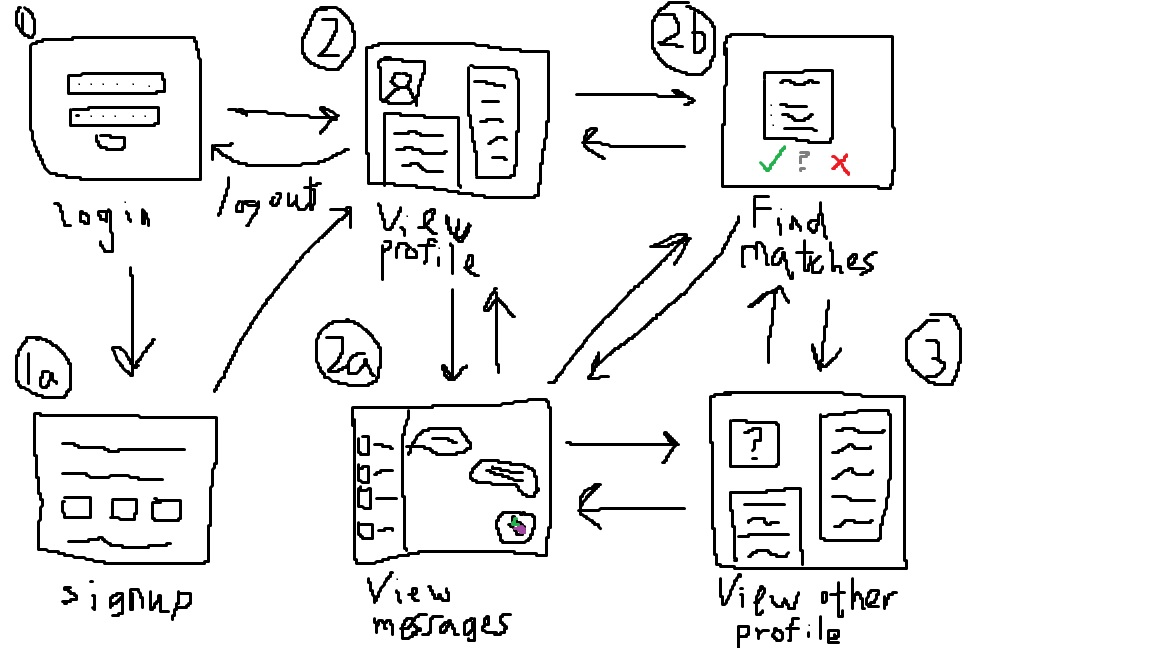
\includegraphics[width=\columnwidth]{storyboard.jpg}$
    \end{enumerate}
\end{document}